
\newpage
\begin{center}
\textbf{\large ГЛАВА 4 \\ «Влияние дальнодействия силя притяжения на скорость нуклеации»}
\end{center}
\refstepcounter{chapter}

\addcontentsline{toc}{chapter}{ГЛАВА 4. Влияние дальнодействия силя притяжения на скорость нуклеации}

\section{Введение}
\label{PRIMe-SecIntroduction}

Построение фазовых диаграмм различных систем является крайне важным для многих направлений науки и техники.
Особую роль фазовые диаграммы играют в области металлургии.
На данный момент удобным инструментом для изучения фазовых состояний веществ на уровне отдельных частиц является метод молекулярной динамики~\cite{10.1063/1.1730376, 10.1006/jcph.1995.1039} и модельные системы, например, пылевая плазма и коллойдные частицы во вращающихся электрических и магнитных полях~\cite{10.1038/s41598-017-14001-y, 10.1103/physreve.103.022608, 10.1103/physreve.96.043201}.
Для построения фазовых диаграмм систем существует несколько способов расчета, которые основаны на знании координат частиц в каждый момент времени.
К ним относятся термодинамическое интегрирование~\cite{10.1088/0953-8984/21/46/465104}, кластеризация с помощью разбиения на ячейки вороного~\cite{10.1021/acs.jpcc.7b09317} и метод вычисления плотности газа и конденсата с помощью расчета профиля плотности системы с зафиксированными в пространстве газовой и конденсированной фазой~\cite{10.1021/jp806127j, 10.1021/jp1117213}.

Однако каждый из этих методов имеет ряд недостатков, которые не позволяют им быть универсальным способом для расчета фазовых диаграмм различных веществ ввиду большого количества параметров для настройки метода или неприменимости метода к кластерам произвольной формы, либо высокая сложность алгоритма.

Данные проблемы могут быть решены с помощью алгоритма кластеризации данных DBSCAN, который впервые применен к молекулярным системам и показал хорошие результаты.
Это открывает возможности для более глубокого изучения зависимости фазовых диаграмм от вида потенциала, для изучения плавления и нуклеации веществ, а также для многих других областей, изучаемых с помощью модельных систем и МД моделирований.


\section{Methods}
\label{PRIMe-SecMethods}

\subsection{Алгоритм кластеризации данных DBSCAN как классификатор частиц в двухфазных системах}
\label{PRIMe-SubSecDBSCAN}

Для решения задачи классификации частиц в двухфазных системах был выбран алгоритм кластеризации DBSCAN.
Выбор данного метода обусловлен тем, что он позволяет классифицировать систему на кластеры данных и выбросы, что в рамках задачи распознавания фаз можно интепретировать как конденсат и газ соответственно.

Для корректной работы данного алгоритма кластеры данных должны быть одинаковой плотности, что в нашем случае соответствует кластерам, находящимся в термодинамическом равновесии друг с другом.
Данный алгоритм естественным образом легко адаптировать как к двумерным, так и к трехмерным системам частиц, что позволяет применять его в широком диапазоне задач мягкой материи.

DBSCAN требует задания двух параметров: $\varepsilon$-окрестность и минимального числа точек $k$, которые должны образовывать плотную область~\cite{schubert2017dbscan}.
Алгоритм начинается с произвольной точки, которая ещё не просматривалась.
Выбирается $\varepsilon$-окрестность точки и, если она содержит достаточно много точек, то есть больше или равно $k$, помечается как кластер, в противном случае точка помечается как поверхность или шум.

Если точка найдена как плотная точка кластера, её $\varepsilon$~-~окрестность также является частью этого кластера.
Следовательно, все точки, найденные в $\varepsilon$~-~окрестности этой точки, добавляются к кластеру.
Этот процесс продолжается, пока не будет найден связный по плотности кластер.
Затем выбирается и обрабатывается новая непосещённая точка, что ведёт к обнаружению следующего кластера или шума (газовых точек).
Следующим шагом точки кластера, не содержащие в своей $\varepsilon$~-~окрестности $k$ или больше соседей, помечаются как точки поверхности.
Принцип кластеризации показан на рисунке~\ref{kepsilon}.

DBSCAN может быть использован с любой функцией расстояния~\cite{ester1996density, schubert2017dbscan} (а так же с функцией похожести или логическим условием)~\cite{10.1023/a:1009745219419}.
Функция расстояния может рассматриваться как дополнительный параметр.
В рамках анализа двухфазной системы частиц мы используем в качестве функции расстояния норму в Евклидовом пространстве.

Новый алгоритм классификации частиц, основанный на DBSCAN, должен разделять систему на 3 класса (на конденсат, газ и поверхность).
Частица считается основной (конденсат), если в ее окрестности $\varepsilon$ находится не меньше $k$ частиц.
Параметр $k$ играет в нашем случае также роль минимального значения размера кластеров в системе.
Частица считается поверхностной, если она является соседней частицей любой из основных частицы, но при этом не имеет нужное количество соседей, чтобы считаться основной.
Выбросом (то есть газом) являются частицы, которые не являются соседями основных частиц. Пример разбиения системы на три класса представлен на рисунке~\ref{DBSCAN-Illustr}(c).

\begin{figure}[!t]
    \centering
    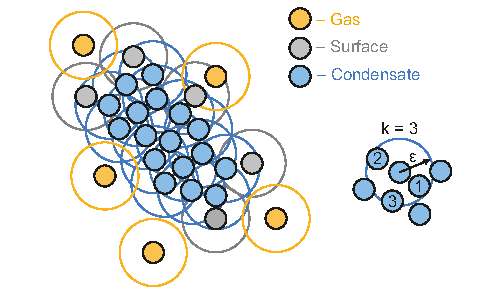
\includegraphics[width=\linewidth]{kepsilon.pdf}
    \caption{Принцип работы алгоритма кластеризации DBSCAN для случая $k = 3$. Синие точки являются основными точками (конденсатом), поскольку область с радиусом $\varepsilon$, окружающая эти точки, содержит по меньшей мере трех соседей (не считая саму точку).
    Серые точки не имеют в своей $\varepsilon$~-~окрестности трех соседей, но имеют покрайней мере одну основную точку (частицу конденсата).
    Такие точки относятся к поверхности.
    Оранжевые точки не имеют в своей $\varepsilon$~-~окрестности ни одну основную точку, поэтому считаются частицами газа.}
    \label{kepsilon}
\end{figure}

Важным вопросом применения данного алгоритма является выбор оптимальных значений параметров $\varepsilon$ и $k$.
В качестве функции расстояния мы используем норму Евклидова пространства, однако выбор $\varepsilon$ и $k$ не так очевиден.

В задачах классификации выбор значения $\varepsilon$ часто выполняется автоматически и зависит только от $k$.
Для каждой точки данных вычисляется расстояние до самой дальней точки, из $k$ самых ближайших.
Полученные расстояния сортируются, и на графике зависимости данного расстояния от индекса массива отсортированных точек наблюдается точка перегиба, которая определяет оптимальное значение параметра $\varepsilon$.
Наиболее эффективным способом ее нахождения является нахождение точки, наиболее удаленной от прямой, соединяющей минимальное и максимальное значение расстояния.
Выбор оптимальных параметров иллюстрируется на рисунке~\ref{epsilon_k}.

Мы обнаружили, что для нашей физической задачи это также хорошо работает, поэтому единственным свободным параметром в нашем алгоритме остается значение $k$, которое имеет смысл минимального значения размера кластера, и как будет показано далее, может быть выбрано в большом диапазоне значений, а малое изменение данного параметра слабо влияет на результат классификации, что делает работу данного метода более стабильной.
Пример кластеризации системы частиц после применения алгоритма DBSCAN представлен на рисунке \ref{DBSCAN-Illustr}(a).

\begin{figure}[!t]
    \centering
    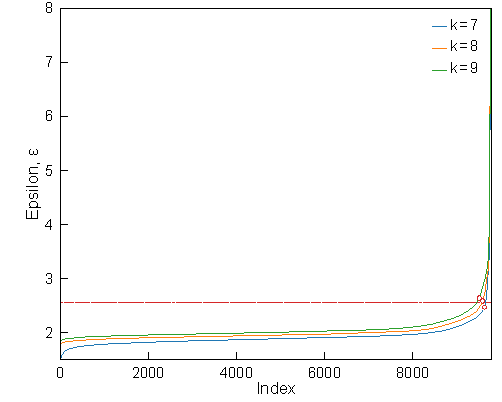
\includegraphics[width=\linewidth]{Figure0.pdf}
    \caption{Выбор оптимального параметра $\varepsilon$. Красным цветом указаны точки для различных значений параметра $k$, наиболее удаленные от линии, соединяющей начало и конец кривой расстояний.}
    \label{epsilon_k}
\end{figure}

Классификация частиц поверхности в зависимости от задачи может быть различной.
При необходимости отнесения к поверхности минимального количества частиц можно считать поверхностью только те частицы, которые относятся к конденсату, но не считаются основными (по условию k-NN < k).
Данное выделение поверхности представлено на рисунке~\ref{DBSCAN-Illustr}(b).
Однако при необходимости выделения поверхности, полностью ограничивающие кластер, может быть применен алгоритм выделения поверхности.
Алгоритм выделения поверхности следующий: используя альфа-формы, набору точек можно присвоить многоугольник с помощью набора кругов определенного радиуса: вокруг точек рисуется произвольная форма, и удаляется как можно больше этой формы, используя круги определенного радиуса.
Это продолжается как можно дольше, не замыкая ни одной точки.
Малый радиус будет означать, что можно удалить больше <<материала>>, больший радиус означает меньшее <<удаление>>, т.е. малый радиус создает плотную обрезанную форму, тогда как бесконечный радиус воссоздает выпуклую оболочку набора.
Точки, определенные как краевые, затем соединяются прямыми гранями.
Это может создать пустые области внутри набора точек.
Система, после применения данного алгоритма выделения поверхности представлена на рисунке~\ref{DBSCAN-Illustr}(c).

\begin{figure*}[!t]
    \centering
    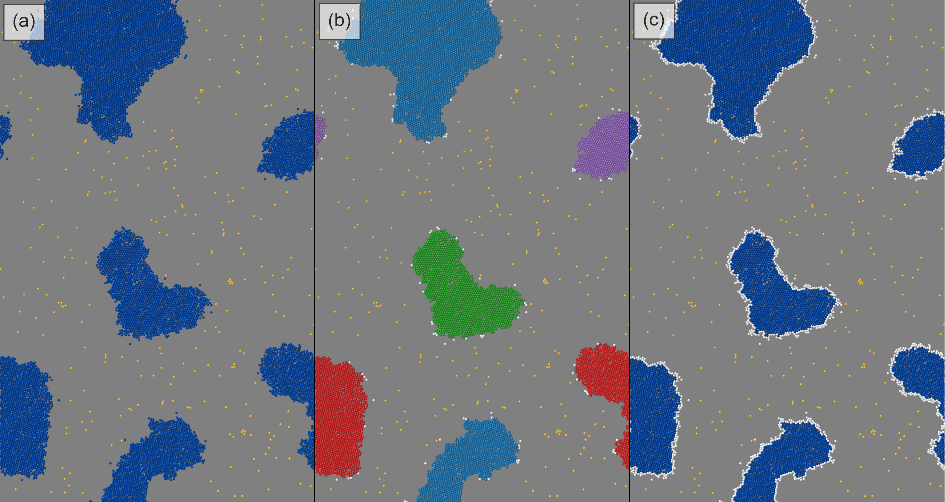
\includegraphics[width=160mm]{PRIMe-Figure104.pdf}
    \caption{Пример распознавания частиц в 2D системе LJ12-6. (a) результат работы метода DBSCAN (классификация частиц на конденсат и газ). (b) пример выделения частиц поверхности, по условию принадлежности к конденсату и не к основным частицам. Разные кластеры раскрашены в разные цвета с учетом регулярных граничных условий. (с) пример выделения регулярной поверхности, охватывающей все частицы кластера.}
    \label{DBSCAN-Illustr}
\end{figure*}

Данный метод легко обобщается на трехмерные системы. Пример классификации частиц в трехмерном моделировании с потенциалом Леннарда-Джонса 12-6 изображен на рисунках \ref{D3_flat_layer} и \ref{D3_free_conf}.

\begin{figure}[!t]
    \centering
    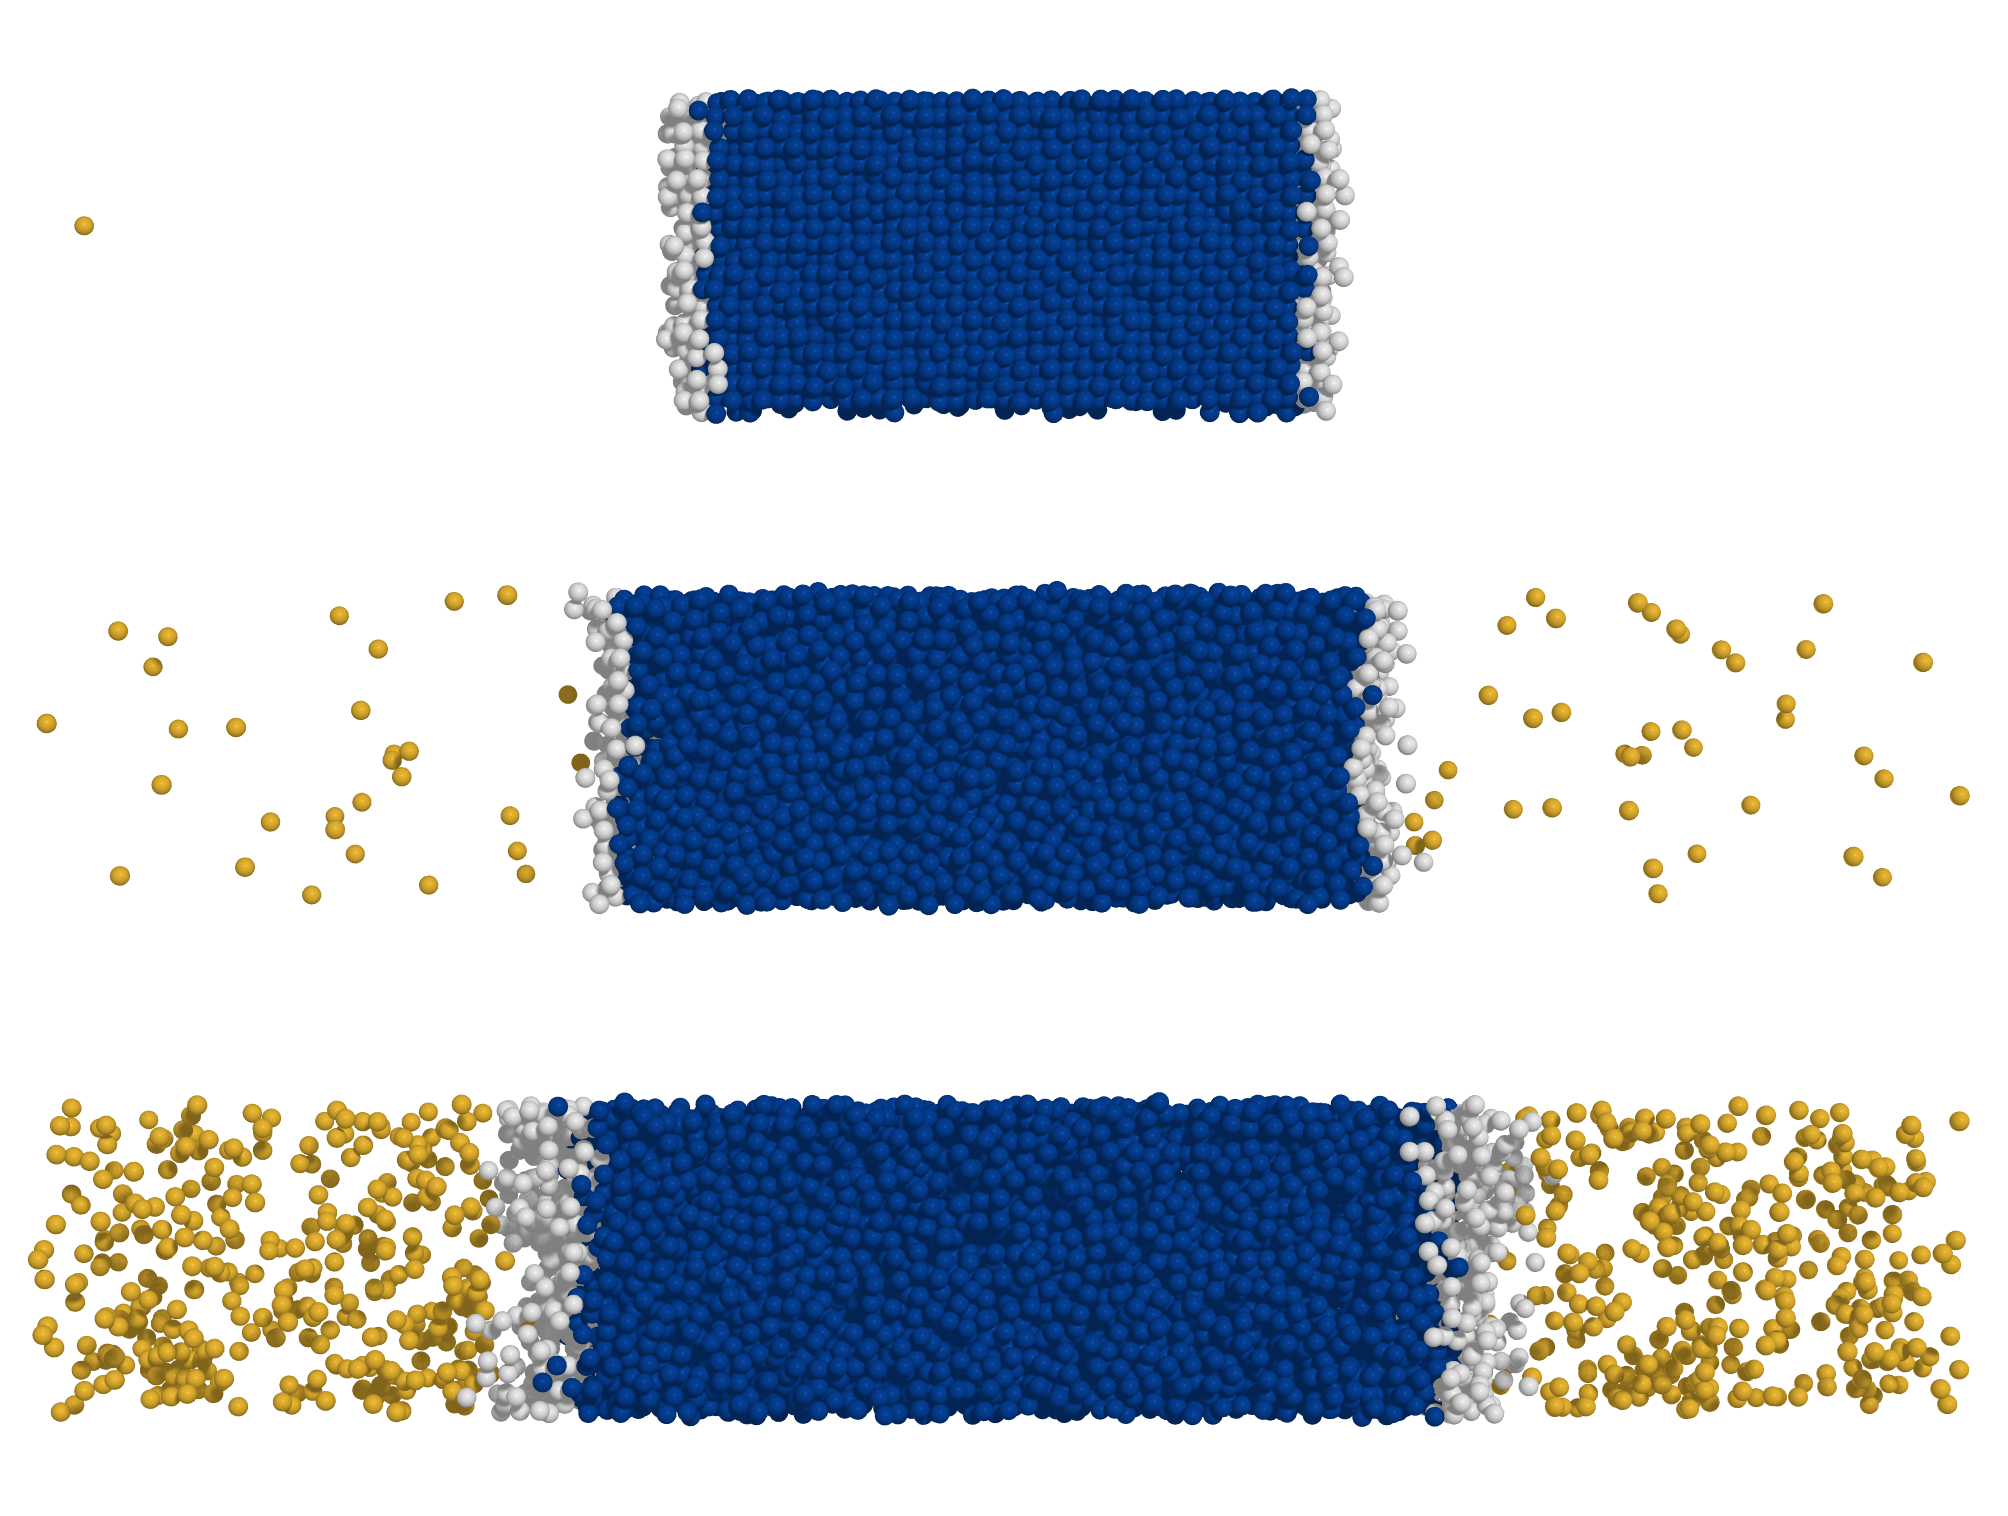
\includegraphics[width=\linewidth]{PRIMe-Figure101.png}
    \caption{Распознавание фаз методом DBSCAN в 3D системе LJ12-6 в случае плоского слоя для разных температур.}
    \label{D3_flat_layer}
\end{figure}


\begin{figure*}[!t]
    \centering
    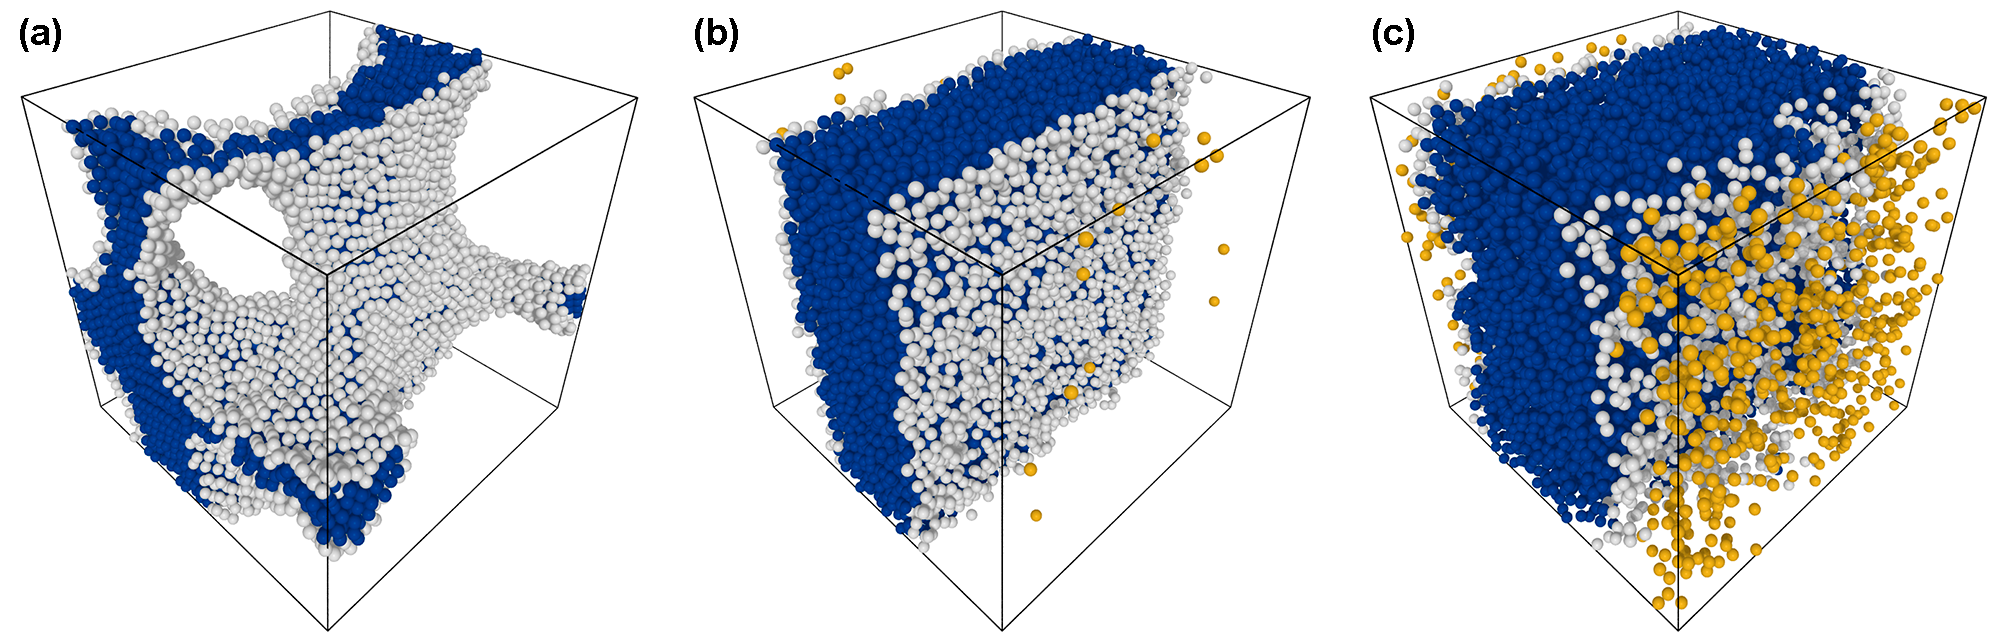
\includegraphics[width=170mm]{PRIMe-Figure103.png}
    \caption{Распознавание фаз для кластера произвольной формы в трехмерной системе LJ12-6 при различной температуре: (a) Кластер произвольной формы при температуре ниже тройной точки; (b) система в состоянии жидкость + газ. (с) система вблизи критической точки.}
    \label{D3_free_conf}
\end{figure*}



\subsection{Построение фазовых диаграмм}
\label{PRIMe-SubSecPhaseDiagram}

Новый метод классификации частиц на фазы дает возможность использовать новый подход к построению фазовых диаграмм, основанный на вычислении плотности подсистем, содержащих только частицы определенной фазы.
Для демонстрации работы нового метода классификации и построения фазовых диаграмм были проведены МД-моделирования в NVT ансамбле системы частиц, взаимодействующих по обобщенному потенциалу Леннарда-Джонса (LJn-m):

\begin{equation}
U_{n-m}(r)=4 \varepsilon\left[\left(\frac{\sigma}{r}\right)^{n}-\left(\frac{\sigma}{r}\right)^{m}\right]
\label{MACR-eq1}
\end{equation}
где $\epsilon$ и $\sigma$ - магнитуда и характерный масштаб отталкивания соответственно.
Мы использовали нормированную температуру $ T/ \epsilon \rightarrow T $, расстояние $ r/ \sigma \rightarrow r $,
плотность частиц $ \rho \sigma ^ 3 / m \rightarrow n$ (здесь $ m $ - масса частицы).

В качестве примеров мы рассмотрели потенциалы LJ12-4, LJ12-5, LJ12-6, LJ16-6 в случае трехмерных, и LJ12-3, LJ12-4, LJ12-5, LJ12-6, LJ12-7 в случае двумерных систем.

После классификации системы на конденсат газ и поверхность мы можем применять данные для различных расчетов, например, вычислять фазовые диаграммы веществ.

Для этого случайным образом разбивается вся система на подобласти и расчитываются их плотности как $\rho_i = N / V$, где $N$ -- количество частиц попавших в сферу (окружность для 2D случая) радиусом $\varepsilon$; $V$ -- объем сферы радиусом $\varepsilon$ (площадь окружности в 2D случае); $i$ -- индекс области.

Затем мы относим случайно выбранные области к конденсату или газу по следующим критериям:
\begin{enumerate}
    \item Если в области $\varepsilon$ находятся только частицы конденсата и их не меньше чем $k$, то эта область является конденсатом;
    \item Если в область попали частицы поверхности, то эта область относится к поверхности и не участвует в статистике плотностей газа и конденсата;
    \item Если в область попали только газовые частицы или в области нет частиц, то эта область считается занимаемой газом.
\end{enumerate}
Затем мы можем рассчитать плотности соответствующих областей и вычислить среднее значение плотности конденсата и газа.

Для расчета фазовых диаграмм вещества в координатах $\rho$-$T$ необходимо знать плотность газа и конденсата при соответствующих температурах.
Для этого в начале моделирования берется температура существенно ниже тройной точки и система релаксирует.
После релаксации температура системы начинает медленно линейно повышаться от температуры релаксации до закритической температуры.
Нагревание происходит медленно, поэтому систему в каждый момент времени можно считать находящейся в состоянии термодинамического равновесия.
Это позволяет быстро найти для каждой температуры соответствующие плотности конденсата и газа усреднив их по нескольким соседним кадрам моделирования.

\begin{figure}[!t]
    \centering
    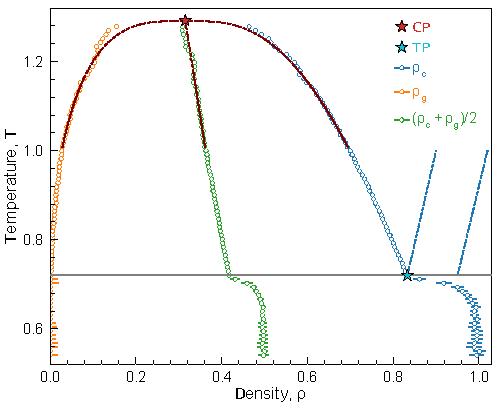
\includegraphics[width=\linewidth]{MACR-Figure2.pdf}
    \caption{Фазовая диаграмма системы LJ12-6, изображенной на рисунке~\ref{D3_free_conf}.
    Оранжевые и синие символы — плотности газа и конденсата, полученные путем усреднения плотности областей, соответствующих конденсату и газу. Зеленые символы -- медиана $\rho_m=(\rho_g+\rho_c)/2$.
    Сплошная красная линия соответствует уравнению ~\eqref{MACR-eq4}.
    Тройные и критические точки обозначены синими и красными звездочками соответственно.}
    \label{phase_diagram}
\end{figure}




% \begin{table}[h!]
%     \centering{
%     \begin{tabular}{>{\centering}p{1.6cm}|>{\centering}p{1.1cm}|>{\centering}p{1.0cm}|>{\centering}p{1.0cm}|>{\centering}p{1.0cm}|>{\centering}p{1.0cm}|>{\centering}p{1.0cm}>{\centering}p{0cm}}
%         Потенциал & $T_{\rm CP}$ & $\rho_{\rm CP}$ & $T_{\rm TP}$ & $\rho_{\rm TP}$ & $A$ & $a$ &\\ \hline
%         \multicolumn{8}{c}{3D системы:} \\ \hline
%         LJ12-4 & 4.416 & 0.278 & 1.500 & 0.980 & 0.578 & 0.128 &\\
%         LJ12-5 & 2.080 & 0.301 & 1.030 & 0.900 & 0.846 & 0.251 &\\
%         LJ12-6 & 1.282 & 0.308 & 0.645 & 0.865 & 1.002 & 0.385 &\\
%         LJ16-6 & 1.532 & 0.309 & 0.900 & 0.850 & 0.987 & 0.412 &\\ \hline
%         \multicolumn{8}{c}{2D системы:} \\ \hline
%         LJ12-3 & 2.697 & 0.304 & 1.080 & 0.820 & 0.702 & 0.117 &\\
%         LJ12-4 & 1.170 & 0.350 & 0.700 & 0.792 & 0.823 & 0.150 &\\
%         LJ12-5 & 0.732 & 0.356 & 0.530 & 0.775 & 0.924 & 0.326 &\\
%         LJ12-6 & 0.517 & 0.355 & 0.405 & 0.780 & 0.982 & 1.019 &\\
%         LJ12-7 & 0.371 & 0.363 & 0.316 & 0.780 & 1.058 & 1.680 &\\ \hline
%     \end{tabular}
%     }
%     \caption{Значения тройных и критических точек, а также коэффициентов фитирования $A$ и $a$ из уравнений \eqref{MACR-eq4} для двумерных и трехмерных систем Леннарда-Джонса, рассматриваемых в данной работе.}
%     \label{PRIMe-Table2}
% \end{table}


Вблизи критической температуры вычисление плотностей газа и конденсата становится затруднительным из-за растущих флуктуаций плотности в системе.
Тем не менее, положение критической точки на фазовой диаграмме может быть рассчитано путем аппроксимации конденсированных и газовых бинодальных ветвей вблизи критической точки следующим образом:
\begin{equation}
    n_{c}-n_{g} \simeq A \tau^{\beta}, \quad n_{c}+n_{g} \simeq a \tau+2 n_{\mathrm{CP}},
\label{MACR-eq4}
\end{equation}
где $\tau=T_{\mathrm{CP}}-T$, $T_{\mathrm{CP}}$ и $n_{\mathrm{CP}}$ - это температура и
плотность в критической точке соответственно, $\beta$ - критический индекс, и $A$ и $a$ являются
параметрами, которые должны быть получены из аппроксимации с $n_{\mathrm{CP}}$ и $T_{\mathrm{CP}}$.
Критический индекс $\beta$ зависит от класса универсальности системы, определяемого межчастичным взаимодействием~\cite{10.1103/physrevlett.89.025703}.

В трехмерии для потенциала LJ12-6 критический индекс $\beta_c = 0.325$, а в случае двумерия $\beta_c = 0.5$.
Пример построения фазовой диаграммы для трехмерной системы LJ12-6 и нахождение тройной и критической точки изображено на рисунке~\ref{phase_diagram}.

Главным достоинством такого подхода к построению фазовых диаграмм по сравнению с методами <<плоского слоя>>~\cite{10.1021/jp806127j, 10.1021/jp1117213} и термодинамическим интегрированием~\cite{10.1088/0953-8984/21/46/465104} является нечувствительность метода к форме кластеров, произвольное начальное и последующее расположение частиц и скорость работы алгоритма благодаря автоматизации выбора параметров и расчетов.



\subsection{Детали МД-моделирований для построения фазовых диаграмм}
\label{PRIMe-SubSecPhaseDiagramMD}



Все МД-симуляции были выполнены в ансамбле NVT (N, V и T - количество частиц, объем системы и температура соответственно) с периодическими граничными условиями с использованием пакета моделирования LAMMPS~\cite{10.1006/jcph.1995.1039}.
Исходное состояние системы формировалось следующим образом: (i) кубический ящик (квадратный в 2D случае) моделирования заполнялся равновесным кристаллом (в нашем случае ГЦК) из $N$ частиц со средней плотностью системы $\rho_a$; (ii) система релаксировала на протяжении $3 \times 10^5$ шагов при температуре $T_{start}$.
Результирующее начальное состояние для 3D системы LJ12-6 показано на рис.~\ref{D3_free_conf}(а).
Затем температура системы линейно увеличивалась от $T_{start}$ до $T_{stop}$ в течение $n_{step}$ шагов моделирования с временным шагом $\Delta t$. Различия в моделированиях представленны в таблице \ref{MACR-Table1}.

%\renewcommand{\arraystretch}{1.25}
% \begin{table}[h!]
%     \centering{
%     \begin{tabular}{>{\centering}p{1.6cm}|>{\centering}p{1.1cm}|>{\centering}p{1.0cm}|>{\centering}p{1.0cm}|>{\centering}p{1.0cm}|>{\centering}p{1.0cm}|>{\centering}p{1.0cm}>{\centering}p{0cm}}
%         Потенциал & $\rho_a$ & $r_c$ & $T_{\rm start}$ & $T_{\rm stop}$ & $n_{step}$& $\Delta t$ &\\  \hline
%         \multicolumn{8}{c}{3D системы:} \\\hline
%         LJ12-4 & \multirow{4}*{0.35} & 12.0 & 0.5 & 4.5 & \multirow{4}*{$5 \times 10^6$}  & \multirow{4}*{$5 \times 10 ^ {- 4}$} &\\
%         LJ12-5 &  & 10.0 & 0.2 & 2.5 & & &\\
%         LJ12-6 &  & 8.0 & 0.4 & 1.4 &  & &\\
%         LJ16-6 &  & 8.0 & 0.6 & 1.6 &  & &\\ \hline
%         \multicolumn{8}{c}{2D системы:} \\\hline
%         LJ12-3 & \multirow{5}*{0.35} & 15.0 & 0.5 & 3.0 & \multirow{5}*{$7 \times 10^6$}  & \multirow{5}*{$5 \times 10 ^ {-4}$} &\\
%         LJ12-4 &  & 15.0 & 0.4 & 1.4 & & &\\
%         LJ12-5 &  & 10.0 & 0.2 & 0.9 &  & &\\
%         LJ12-6 &  & 8.0 & 0.35 & 0.55 &  & &\\
%         LJ12-7 &  & 8.0 & 0.28 & 0.4 &  & &\\ \hline
%     \end{tabular}
%     }
%     \caption{Параметры, используемые в МД-моделировании для бимодальных расчетов:
%     где $\rho$ — средняя плотность системы, $r_c$ — радиус отсечки,
%     $T_{start}$ и $T_{stop}$ — начальная и конечная температуры моделирования,
%     $n_{step}$ — количество шагов моделирования, а
%     $\Delta t$ — временной шаг.}
%     \label{MACR-Table1}
% \end{table}
%
\section{Результаты}
\label{PRIMe-SecResults}

\subsection{Результаты построения фазовых диаграмм}
\label{PRIMe-SubSecPhaseDiagramMD}

На рисунке \ref{phase_diagram}(a) и \ref{phase_diagram}(b) представленны результаты построения фазовых диаграмм для двумерия и трехмерия соответственно, расчитанные с помощью нового метода классификации частиц на фазы.
Фазовые диаграммы нормированны на температуру и плотность тройной точки, представленные в таблице \ref{PRIMe-Table2}.

Как можно заметить, представленные фазовые диаграммы имеют стабильный результат с небольшим значением шумов плотности конденсата и газа.
Данный результат показывает большую стабильность по сравнению с другим методом построения фазовых диаграмм,  метода плоского слоя, описанного в работах~\cite{10.1021/jp806127j, 10.1021/jp1117213}.
Важным достоинством нового метода построения фазовых диаграмм является то, что для расчета не требуется множество моделирований как для метода термодинамического интегрирования~\cite{10.1080/00268976.2019.1699185}, либо системы конкретной формы, как для моделирования плоского слоя~\cite{10.1021/jp806127j, 10.1021/jp1117213}.
В таблице~\ref{PRIMe-Table3} приведена сравнительная таблица нового метода с другими методами построения фазовых диаграмм.


%
% \begin{table}[h!]
%     \centering{
%     \begin{tabular}{>{\centering}p{3.0cm}|>{\centering}p{1.0cm}|>{\centering}p{0.7cm}|>{\centering}p{1.5cm}|>{\centering}p{1.5cm}>{\centering}p{0cm}}
%         Метод & Форма & 3D & Скорость & Точность &\\  \hline
%         Представленный метод & \checkmark & \checkmark & \checkmark & \checkmark & \\
%         Метод плоского слоя~\cite{10.1021/jp806127j, 10.1021/jp1117213} & $\times$ & \checkmark & \checkmark & $\times$ & \\
%         Термодинамическое интегрирование~\cite{10.1080/00268976.2019.1699185} & \checkmark   & \checkmark   & $\times$   & \checkmark   & \\
%         Метод основанный на $R^2$-параметре~\cite{10.1021/acs.jpcc.7b09317} & \checkmark & $\times$ & \checkmark & $\times$ & \\ \hline
%     \end{tabular}
%     }
%     \caption{Сравнение различных методов построения фазовых диаграмм. Под 2D и 3D понимается применимость данных методов в двумерных или трехмерных системах; под скоростью подразумевается величина затраченого времени в человеко-часах на одну точку фазовой диаграммы относительно других представленных методов; под точностью понимается точность метода относительно других представленных методов.}
%     \label{PRIMe-Table3}
% \end{table}



\begin{figure*}[!t]
    \centering
    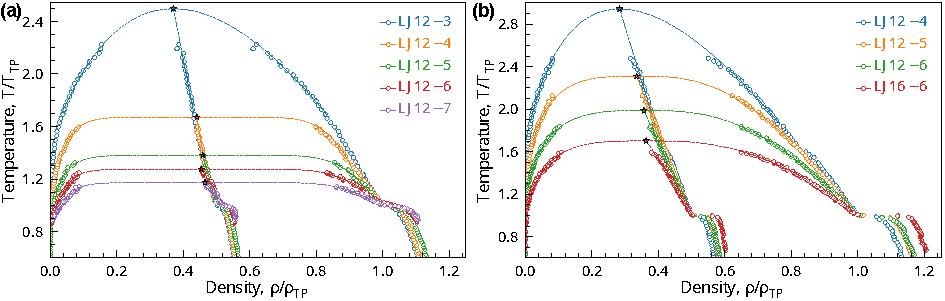
\includegraphics[width=160mm]{Figure11.pdf}
    \caption{Фазовые диаграммы систем с различным дальнодействием притяжения.
    (a) Фазовые диаграммы в двумерных системах.
    (b) Фазовые диаграммы в трехмерных системах.}
    \label{phase_diagram}
\end{figure*}

\subsection{Тесты на устойчивость метода к плотности системы и входным параметрам}
\label{PRIMe-SubSecTests}


Для успешного применения данного алгоритма кластеризации необходимо понимать его границы применимости.
Для этого были проведены тесты на устойчивость метода к изменению начальной плотности системы и выбору минимального размера кластеров.

\begin{figure*}[!t]
    \centering
    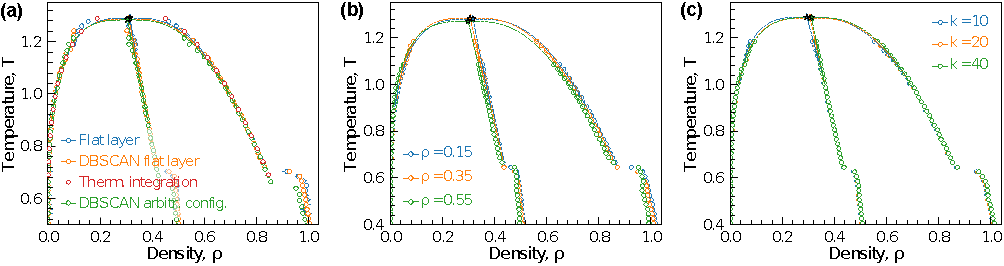
\includegraphics[width=\linewidth]{Figure10.pdf}
    \caption{\textbf{(a)} Сравнение различных методов построения фазовых диаграмм. Красным отмечен самый точный метод - термодинамическое интегрирование~\cite{10.1080/00268976.2019.1699185}.
             \textbf{(b)} Тест на влияние средней плотности на фазовую диаграмму системы LJ12-6 в трехмерии.
             \textbf{(c)} Тест на влияние начального параметра $k$ на фазовую диаграмму системы LJ12-6 в трехмерии.}
    \label{tests}
\end{figure*}



На рисунке~\ref{tests}(b) представлен результат построения фазовых диаграмм систем с потенциалом взаимодействия LJ12-6 в трехмерии с различной начальной плотностью системы. Как можно заметить, существенное изменение плотности системы слабо влияет на расчет фазовых диаграмм и критических точек.



Кроме устойчивости к плотности системы данный алгоритм построения фазовых диаграмм должен также быть нечувствительным к изменению параметра $k$.
На рисунке~\ref{tests}(c) продемонстрирован тест на чувствительность метода к данному параметру.
Была смоделирована система с потенциалом LJ12-6 в трехмерии, и новым методом расчета.
Были построены фазовые диаграммы с использованием различных входных параметров $k$.
Анализ результатов показывает, что изменение параметра $k$ практически не влияет на фазовую диаграмму.



Для сравнения нашего метода с другими методами построения фазовых диаграмм была проведена обработка одного моделирования нашим методом и методом <<плоского слоя>>~\cite{10.1021/jp806127j, 10.1021/jp1117213}.
Кроме того, данные результаты были сравнены с фазовой диаграммой системы с произвольной начальной формой кластера.
Результаты тестов приведены на рисунке~\ref{tests}(a), где синим цветом обозначена фазовая диаграмма вычисленная методом <<плоского слоя>>, оранжевым цветом обозначена фазовая диаграмма рассчитанная новым методом распознавания фаз, но на том же моделировании, что и <<плоский слой>>, и зеленым цветом показана фазовая диаграмма вычисленная новым методом, но на моделировании с произвольным начальным расположением частиц. Красным цветом представленны данные, расчитанные методом термодинамического интегрировния, самым точным из представленных~\cite{10.1080/00268976.2019.1699185}.

Как можно заметить, фазовая диаграмма, построенная по моделированию, содержащему плоский слой частиц оказалась практически идентичной для разных методов.
Причем новый метод дает более плавную фазовую диаграмму и меньшую погрешность плотности кристаллической фазы.
Однако новый метод, примененный к системе с произвольным расположением частиц, дает несколько отличный результат от методов, примененных к плоскому слою частиц.
Это связано с тем, что <<плоский слой>> частиц более стабильный и может находится в состоянии перегретого кристалла, в то время как на кластерах произвольной формы зародыши плавления начинают появляться при меньшей температуре.
Данный факт делает <<плоский слой>> не таким универсальным методом, как новый метод классификации основанный на DBSCAN, так как результирующие фазовые диаграммы полученные методом плоского слоя имеют завышенную тройную точку, в отличии от нового метода, который способен строить фазовую диаграмму для систем с произвольной формой.


\section{Изучения скорости нуклеации в переохлажденных системах}
\label{PRIMe-SecNucleation}

Для демонстрации возможностей нового метода распознавания фаз была выбрана задача определения влияния дальнодействия потенциала на скорость нуклеации в системе с одинаковой степенью переохлаждения.

Для того, чтобы исключить влияние глубины потенциальной ямы на скорость нуклеации, был выбран следующий потенциал:
\begin{equation}
U_{nm}(r)=\frac{\epsilon}{n-m}\left(\frac{m}{r^n}-\frac{n}{r^m}\right) \label{NMP-eq1}
\end{equation}
При данном потенциале взаимодействия глубина остается постоянно равной единицы, в то время как дальнодействие можно изменять варьируя степень притяжения $m$.

Для выяснения степени переохлаждения системы были вычислены температурные точки для двумерных систем $U_{12-4}$, $U_{12-5}$, $U_{12-6}$, $U_{12-7}$. Значение температуры тройной точки определяется по резкому уменьшению плотности бинодали жидкость-газ.

Затем моделируются системы с равномерной плотностью распределения частиц и одинаковой степенью переохлаждения, то есть температура моделирования есть $T = T_{TP} / a$, где в рамках нашей задачи $a = 3.0$, а $T_{TP}$ - температура тройной точки, вычисляется на предыдущем шаге.

На рисунке~\ref{otchet} представлены снимки системы через разное время после начала моделирования. Новый алгоритм классификации на фазы позволяет наблюдать за процессами зарождения и последующего <<слипания>> кластеров.



\begin{figure*}[!t]
	 \centering
	 \includegraphics[width=170mm]{otchet.pdf}
	 \caption{Процесс зарождения и роста кластеров в переохлажденной системе частиц взаимодействующих посредством потенциала Леннарда-Джонса.}
	 \label{otchet}
\end{figure*}


\begin{figure}[!t]
    \centering
    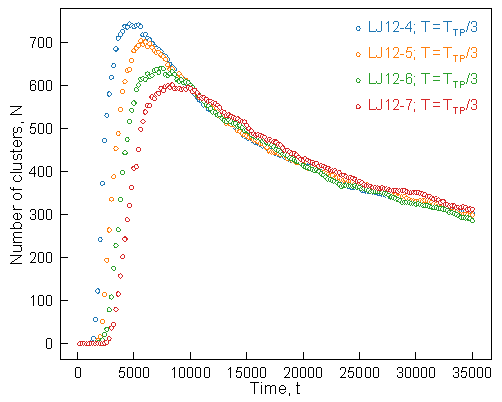
\includegraphics[width=\linewidth]{countCluster.pdf}
    \caption{Зависимость количества кластеров от времени.}
    \label{countCluster}
\end{figure}

На рисунке~\ref{countCluster} показана временная зависимость количества кластеров в системах с различным дальнодействием притяжения. Можно заметить, что дальнодействие притяжения существенно влияет на начальные этапы нуклеации, но дальнейшее увеличение кластеров посредством слипания никак не зависит от дальнодействия. Существенное отличие графиков на начальном этапе можно объяснить тем, что дальнодействие потенциала позволяет быстрее собраться частицам в кластер нужного размера для попадания в статистику, так как кластерами в данном алгоритме считаются только те скопления частиц, которые больше критического, то есть $k = 9$.

\begin{figure}[!t]
    \centering
    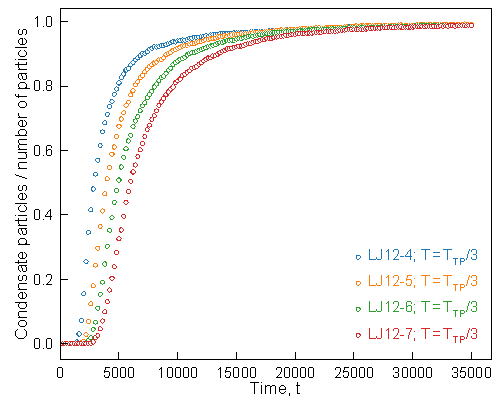
\includegraphics[width=\linewidth]{countParticles.pdf}
    \caption{Зависимость доли частиц, находящихся в конденсированном состоянии от времени для различных потенциалов.}
    \label{countParticles}
\end{figure}

На рисунке~\ref{countParticles} показана временная зависимость доли частиц, находящихся в конденсированном состоянии. Видно, что скорость, с которой частицы становятся частицами кластера, зависит от дальнодействия потенциала. Закономерно, что в случае более дальнодействующего потенциала частицы слипаются быстрее, чем при короткодействующем.

\begin{figure}[!t]
    \centering
    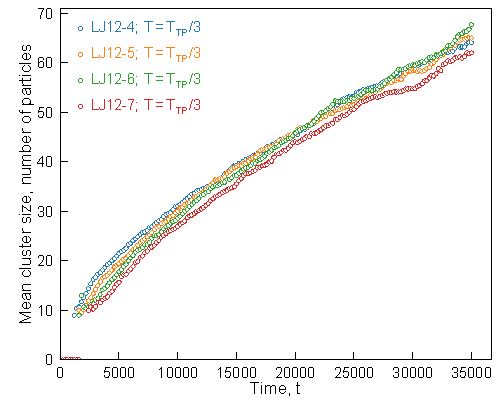
\includegraphics[width=\linewidth]{meanParticles.pdf}
    \caption{Зависимость среднего размера кластера от времени для систем с различным дальнодействием потенциала.}
    \label{meanParticles}
\end{figure}

На рисунке~\ref{meanParticles} изображена зависимость среднего размера кластера от времени. Как можно заметить, дальнейший рост кристаллов слабо зависит от дальнодействия потенциала, и наклон зависимости среднего количества частиц одинаков для всех рассматриваемых потенциалов.


%
% \newpage
%
% \section*{Appendix}
% \label{MACR-SecAppendix}
%
%
% \begin{table*}[]
% \centering
% \begin{tabular}{p{0.4cm}|p{1.4cm}p{1.4cm}p{1.4cm}p{1.4cm}p{1.4cm}p{1.4cm}p{1.4cm}p{1.4cm}p{1.4cm}p{1.4cm}p{1.4cm}}
% \multicolumn{11}{c}{LJ12-3, 2D}  \\ \hline\hline
% $T$   &  0.509   &  0.545   &  0.580   &  0.616   &  0.652   &  0.688   &  0.723   &  0.759   &  0.795   &  0.830   &  0.866  \\
% $\rho_c$   &  0.917   &  0.915   &  0.910   &  0.907   &  0.906   &  0.904   &  0.899   &  0.898   &  0.892   &  0.888   &  0.885  \\
% $\rho_g$   &  1.00e-06   &  0.00e+00   &  1.00e-06   &  4.00e-06   &  4.00e-06   &  1.70e-05   &  7.00e-06   &  6.30e-05   &  4.50e-05   &  6.40e-05   &  6.50e-05  \\ \hline\hline
% $T$   &  0.902   &  0.938   &  0.973   &  1.009   &  1.045   &  1.080   &  1.116   &  1.152   &  1.188   &  1.223   &  1.259  \\
% $\rho_c$   &  0.881   &  0.874   &  0.869   &  0.861   &  0.852   &  0.825   &  0.812   &  0.803   &  0.797   &  0.791   &  0.783  \\
% $\rho_g$   &  1.27e-04   &  1.63e-04   &  2.32e-04   &  2.16e-04   &  4.14e-04   &  9.28e-04   &  8.44e-04   &  1.49e-03   &  1.66e-03   &  2.60e-03   &  2.92e-03  \\ \hline\hline
% $T$   &  1.295   &  1.330   &  1.366   &  1.402   &  1.438   &  1.473   &  1.509   &  1.545   &  1.580   &  1.616   &  1.652  \\
% $\rho_c$   &  0.779   &  0.774   &  0.764   &  0.759   &  0.753   &  0.748   &  0.742   &  0.733   &  0.729   &  0.721   &  0.714  \\
% $\rho_g$   &  3.70e-03   &  3.70e-03   &  5.34e-03   &  6.26e-03   &  6.82e-03   &  8.28e-03   &  9.57e-03   &  1.15e-02   &  1.16e-02   &  1.30e-02   &  1.66e-02  \\ \hline\hline
% $T$   &  1.688   &  1.723   &  1.759   &  1.795   &  1.830   &  1.866   &  1.902   &  1.938   &  1.973   &  2.009   &  2.045  \\
% $\rho_c$   &  0.711   &  0.702   &  0.692   &  0.683   &  0.679   &  0.669   &  0.662   &  0.656   &  0.648   &  0.635   &  0.628  \\
% $\rho_g$   &  1.72e-02   &  2.04e-02   &  2.32e-02   &  2.67e-02   &  3.20e-02   &  3.44e-02   &  3.79e-02   &  4.30e-02   &  4.84e-02   &  5.20e-02   &  5.60e-02  \\ \hline\hline
% $T$   &  2.080   &  2.116   &  2.152   &  2.188   &  2.223   &  2.259   &  2.295   &  2.330   &  2.366   &  2.402   &     \\
% $\rho_c$   &  0.620   &  0.606   &  0.600   &  0.584   &  0.569   &  0.565   &  0.545   &  0.537   &  0.501   &  0.509   &     \\
% $\rho_g$   &  6.04e-02   &  6.87e-02   &  7.46e-02   &  8.19e-02   &  9.41e-02   &  9.68e-02   &  1.09e-01   &  1.22e-01   &  1.25e-01   &  1.27e-01   &     \\ \hline\hline
% \end{tabular}
% \caption{Значения температуры и соотвествующих плотностей газа и конденсата на фазовой диаграмме для двумерной системы LJ12-3}
% \label{MACR-TableLJ2D12-3}
% \end{table*}
%
%
% \begin{table*}[]
% \centering
% \begin{tabular}{p{0.4cm}|p{1.4cm}p{1.4cm}p{1.4cm}p{1.4cm}p{1.4cm}p{1.4cm}p{1.4cm}p{1.4cm}p{1.4cm}p{1.4cm}p{1.4cm}}
% \multicolumn{11}{c}{LJ12-4, 2D}  \\ \hline\hline
% $T$   &  0.404   &  0.418   &  0.432   &  0.446   &  0.461   &  0.475   &  0.489   &  0.504   &  0.518   &  0.532   &  0.546  \\
% $\rho_c$   &  0.883   &  0.880   &  0.878   &  0.879   &  0.875   &  0.874   &  0.872   &  0.869   &  0.866   &  0.865   &  0.861  \\
% $\rho_g$   &  5.10e-05   &  0.00e+00   &  2.80e-05   &  1.70e-05   &  1.90e-05   &  8.80e-05   &  7.90e-05   &  6.70e-05   &  2.51e-04   &  7.70e-05   &  2.27e-04  \\ \hline\hline
% $T$   &  0.561   &  0.575   &  0.589   &  0.604   &  0.618   &  0.632   &  0.646   &  0.661   &  0.675   &  0.689   &  0.704  \\
% $\rho_c$   &  0.860   &  0.858   &  0.855   &  0.850   &  0.848   &  0.844   &  0.841   &  0.839   &  0.834   &  0.827   &  0.806  \\
% $\rho_g$   &  4.95e-04   &  3.27e-04   &  4.33e-04   &  8.03e-04   &  1.02e-03   &  1.04e-03   &  1.44e-03   &  1.45e-03   &  1.82e-03   &  2.50e-03   &  2.85e-03  \\ \hline\hline
% $T$   &  0.718   &  0.732   &  0.746   &  0.761   &  0.775   &  0.789   &  0.804   &  0.818   &  0.832   &  0.846   &  0.861  \\
% $\rho_c$   &  0.787   &  0.781   &  0.779   &  0.772   &  0.765   &  0.764   &  0.757   &  0.754   &  0.748   &  0.738   &  0.740  \\
% $\rho_g$   &  3.32e-03   &  4.16e-03   &  4.32e-03   &  4.93e-03   &  5.83e-03   &  7.75e-03   &  7.93e-03   &  9.51e-03   &  1.02e-02   &  1.15e-02   &  1.36e-02  \\ \hline\hline
% $T$   &  0.875   &  0.889   &  0.904   &  0.918   &  0.932   &  0.946   &  0.961   &  0.975   &  0.989   &  1.004   &  1.018  \\
% $\rho_c$   &  0.735   &  0.730   &  0.722   &  0.719   &  0.718   &  0.704   &  0.704   &  0.700   &  0.694   &  0.692   &  0.685  \\
% $\rho_g$   &  1.24e-02   &  1.56e-02   &  1.77e-02   &  1.77e-02   &  2.09e-02   &  2.35e-02   &  2.35e-02   &  2.70e-02   &  3.22e-02   &  3.42e-02   &  3.75e-02  \\ \hline\hline
% $T$   &  1.032   &  1.046   &  1.061   &  1.075   &  1.089   &  1.104   &  1.118   &  1.132   &  1.146   &  1.161   &  1.175  \\
% $\rho_c$   &  0.675   &  0.670   &  0.666   &  0.657   &  0.646   &  0.644   &  0.633   &  0.633   &  0.622   &  0.605   &  0.589  \\
% $\rho_g$   &  3.95e-02   &  4.27e-02   &  4.70e-02   &  4.95e-02   &  5.42e-02   &  6.28e-02   &  6.81e-02   &  7.22e-02   &  7.42e-02   &  7.61e-02   &  8.10e-02  \\ \hline\hline
% $T$   &  1.189   &  1.204   &  1.218   &  1.232   &  1.246   &  1.261   &  1.275   &  1.289   &  1.304   &  1.318   &  1.332  \\
% $\rho_c$   &  0.589   &  0.573   &  0.553   &  0.530   &  0.527   &  0.513   &  0.491   &  0.478   &  0.471   &  0.456   &  0.461  \\
% $\rho_g$   &  8.77e-02   &  8.01e-02   &  8.49e-02   &  8.68e-02   &  8.81e-02   &  8.84e-02   &  8.53e-02   &  7.71e-02   &  7.72e-02   &  7.65e-02   &  7.41e-02  \\ \hline\hline
% $T$   &  1.346   &  1.361   &  1.375   &  1.389   &      &      &      &      &      &      &     \\
% $\rho_c$   &  0.460   &  0.459   &  0.462   &  0.452   &      &      &      &      &      &      &     \\
% $\rho_g$   &  8.71e-02   &  9.34e-02   &  8.79e-02   &  8.89e-02   &      &      &      &      &      &      &     \\ \hline\hline
% \end{tabular}
% \caption{Значения температуры и соотвествующих плотностей газа и конденсата на фазовой диаграмме для двумерной системы LJ12-4}
% \label{MACR-TableLJ2D12-4}
% \end{table*}
%
%
% \begin{table*}[]
% \centering
% \begin{tabular}{p{0.4cm}|p{1.4cm}p{1.4cm}p{1.4cm}p{1.4cm}p{1.4cm}p{1.4cm}p{1.4cm}p{1.4cm}p{1.4cm}p{1.4cm}p{1.4cm}}
% \multicolumn{11}{c}{LJ12-5, 2D}  \\ \hline\hline
% $T$   &  0.203   &  0.212   &  0.223   &  0.233   &  0.242   &  0.253   &  0.263   &  0.273   &  0.282   &  0.292   &  0.302  \\
% $\rho_c$   &  0.897   &  0.896   &  0.895   &  0.892   &  0.890   &  0.884   &  0.888   &  0.887   &  0.884   &  0.882   &  0.882  \\
% $\rho_g$   &  0.00e+00   &  0.00e+00   &  0.00e+00   &  0.00e+00   &  0.00e+00   &  0.00e+00   &  0.00e+00   &  0.00e+00   &  1.50e-05   &  2.00e-05   &  0.00e+00  \\ \hline\hline
% $T$   &  0.312   &  0.323   &  0.333   &  0.343   &  0.352   &  0.362   &  0.372   &  0.383   &  0.393   &  0.403   &  0.412  \\
% $\rho_c$   &  0.880   &  0.878   &  0.876   &  0.874   &  0.874   &  0.871   &  0.870   &  0.866   &  0.863   &  0.862   &  0.859  \\
% $\rho_g$   &  1.10e-04   &  7.80e-05   &  6.80e-05   &  2.34e-04   &  2.14e-04   &  3.97e-04   &  4.07e-04   &  2.72e-04   &  4.60e-04   &  6.85e-04   &  9.26e-04  \\ \hline\hline
% $T$   &  0.422   &  0.432   &  0.443   &  0.453   &  0.463   &  0.472   &  0.482   &  0.492   &  0.502   &  0.512   &  0.522  \\
% $\rho_c$   &  0.857   &  0.855   &  0.851   &  0.849   &  0.847   &  0.845   &  0.839   &  0.835   &  0.829   &  0.818   &  0.796  \\
% $\rho_g$   &  1.28e-03   &  1.14e-03   &  1.55e-03   &  1.52e-03   &  2.24e-03   &  3.19e-03   &  3.71e-03   &  4.29e-03   &  4.63e-03   &  6.31e-03   &  7.09e-03  \\ \hline\hline
% $T$   &  0.532   &  0.542   &  0.552   &  0.562   &  0.573   &  0.583   &  0.593   &  0.603   &  0.613   &  0.623   &  0.632  \\
% $\rho_c$   &  0.780   &  0.773   &  0.759   &  0.756   &  0.753   &  0.749   &  0.740   &  0.734   &  0.734   &  0.727   &  0.714  \\
% $\rho_g$   &  6.93e-03   &  9.91e-03   &  1.05e-02   &  1.37e-02   &  1.34e-02   &  1.81e-02   &  1.88e-02   &  1.95e-02   &  2.43e-02   &  2.84e-02   &  2.80e-02  \\ \hline\hline
% $T$   &  0.642   &  0.652   &  0.662   &  0.672   &  0.682   &  0.693   &  0.703   &      &      &      &     \\
% $\rho_c$   &  0.708   &  0.703   &  0.702   &  0.695   &  0.678   &  0.671   &  0.663   &      &      &      &     \\
% $\rho_g$   &  3.23e-02   &  3.53e-02   &  3.50e-02   &  4.02e-02   &  4.14e-02   &  5.35e-02   &  5.82e-02   &      &      &      &     \\ \hline\hline
% \end{tabular}
% \caption{Значения температуры и соотвествующих плотностей газа и конденсата на фазовой диаграмме для двумерной системы LJ12-5}
% \label{MACR-TableLJ2D12-5}
% \end{table*}
%
%
% \begin{table*}[]
% \centering
% \begin{tabular}{p{0.4cm}|p{1.4cm}p{1.4cm}p{1.4cm}p{1.4cm}p{1.4cm}p{1.4cm}p{1.4cm}p{1.4cm}p{1.4cm}p{1.4cm}p{1.4cm}}
% \multicolumn{11}{c}{LJ12-6, 2D}  \\ \hline\hline
% $T$   &  0.351   &  0.354   &  0.356   &  0.359   &  0.362   &  0.365   &  0.368   &  0.371   &  0.374   &  0.376   &  0.379  \\
% $\rho_c$   &  0.859   &  0.857   &  0.858   &  0.857   &  0.856   &  0.854   &  0.852   &  0.852   &  0.849   &  0.849   &  0.848  \\
% $\rho_g$   &  4.04e-03   &  4.24e-03   &  4.11e-03   &  5.45e-03   &  5.99e-03   &  5.93e-03   &  7.10e-03   &  6.88e-03   &  6.74e-03   &  7.26e-03   &  7.76e-03  \\ \hline\hline
% $T$   &  0.382   &  0.385   &  0.388   &  0.391   &  0.394   &  0.396   &  0.399   &  0.402   &  0.405   &  0.408   &  0.411  \\
% $\rho_c$   &  0.845   &  0.842   &  0.842   &  0.843   &  0.834   &  0.832   &  0.823   &  0.815   &  0.808   &  0.800   &  0.792  \\
% $\rho_g$   &  8.66e-03   &  9.01e-03   &  9.55e-03   &  1.06e-02   &  1.05e-02   &  1.17e-02   &  1.29e-02   &  1.33e-02   &  1.50e-02   &  1.61e-02   &  1.70e-02  \\ \hline\hline
% $T$   &  0.414   &  0.416   &  0.419   &  0.422   &  0.425   &  0.428   &  0.431   &  0.434   &  0.436   &  0.439   &  0.442  \\
% $\rho_c$   &  0.783   &  0.774   &  0.767   &  0.765   &  0.761   &  0.761   &  0.756   &  0.753   &  0.754   &  0.745   &  0.745  \\
% $\rho_g$   &  1.66e-02   &  1.87e-02   &  1.94e-02   &  2.16e-02   &  2.38e-02   &  2.22e-02   &  2.26e-02   &  2.72e-02   &  2.91e-02   &  2.66e-02   &  2.88e-02  \\ \hline\hline
% $T$   &  0.445   &  0.448   &  0.451   &  0.454   &  0.456   &  0.459   &  0.462   &  0.465   &  0.468   &  0.471   &  0.474  \\
% $\rho_c$   &  0.743   &  0.734   &  0.736   &  0.728   &  0.731   &  0.728   &  0.726   &  0.718   &  0.719   &  0.711   &  0.713  \\
% $\rho_g$   &  3.23e-02   &  3.14e-02   &  3.38e-02   &  3.48e-02   &  3.81e-02   &  3.79e-02   &  4.15e-02   &  4.17e-02   &  4.46e-02   &  4.25e-02   &  4.61e-02  \\ \hline\hline
% $T$   &  0.476   &  0.479   &  0.482   &  0.485   &  0.488   &  0.491   &  0.494   &  0.496   &  0.499   &  0.502   &  0.505  \\
% $\rho_c$   &  0.709   &  0.703   &  0.687   &  0.689   &  0.687   &  0.679   &  0.681   &  0.663   &  0.658   &  0.656   &  0.650  \\
% $\rho_g$   &  4.73e-02   &  5.49e-02   &  5.44e-02   &  5.32e-02   &  5.82e-02   &  6.25e-02   &  6.38e-02   &  5.64e-02   &  6.24e-02   &  6.27e-02   &  6.83e-02  \\ \hline\hline
% $T$   &  0.508   &  0.511   &  0.514   &  0.516   &  0.519   &  0.522   &  0.525   &  0.528   &  0.531   &  0.534   &  0.536  \\
% $\rho_c$   &  0.642   &  0.633   &  0.626   &  0.604   &  0.605   &  0.594   &  0.612   &  0.583   &  0.582   &  0.573   &  0.561  \\
% $\rho_g$   &  6.47e-02   &  6.48e-02   &  6.32e-02   &  6.48e-02   &  6.74e-02   &  6.39e-02   &  6.64e-02   &  6.54e-02   &  6.00e-02   &  6.38e-02   &  6.94e-02  \\ \hline\hline
% $T$   &  0.539   &  0.542   &  0.545   &  0.548   &      &      &      &      &      &      &     \\
% $\rho_c$   &  0.553   &  0.540   &  0.525   &  0.541   &      &      &      &      &      &      &     \\
% $\rho_g$   &  6.54e-02   &  6.40e-02   &  6.11e-02   &  6.75e-02   &      &      &      &      &      &      &     \\ \hline\hline
% \end{tabular}
% \caption{Значения температуры и соотвествующих плотностей газа и конденсата на фазовой диаграмме для двумерной системы LJ12-6}
% \label{MACR-TableLJ2D12-6}
% \end{table*}
%
%
%
% \begin{table*}[]
% \centering
% \begin{tabular}{p{0.4cm}|p{1.4cm}p{1.4cm}p{1.4cm}p{1.4cm}p{1.4cm}p{1.4cm}p{1.4cm}p{1.4cm}p{1.4cm}p{1.4cm}p{1.4cm}}
% \multicolumn{11}{c}{LJ12-7, 2D}  \\ \hline\hline
% $T$   &  0.280   &  0.282   &  0.284   &  0.286   &  0.287   &  0.289   &  0.291   &  0.292   &  0.294   &  0.296   &  0.298  \\
% $\rho_c$   &  0.863   &  0.863   &  0.861   &  0.860   &  0.863   &  0.861   &  0.856   &  0.858   &  0.856   &  0.853   &  0.853  \\
% $\rho_g$   &  8.51e-03   &  8.78e-03   &  1.04e-02   &  1.04e-02   &  1.04e-02   &  1.07e-02   &  1.20e-02   &  1.36e-02   &  1.39e-02   &  1.47e-02   &  1.53e-02  \\ \hline\hline
% $T$   &  0.299   &  0.301   &  0.303   &  0.304   &  0.306   &  0.308   &  0.310   &  0.311   &  0.313   &  0.315   &  0.316  \\
% $\rho_c$   &  0.850   &  0.849   &  0.849   &  0.845   &  0.839   &  0.838   &  0.832   &  0.821   &  0.818   &  0.799   &  0.784  \\
% $\rho_g$   &  1.56e-02   &  1.79e-02   &  1.87e-02   &  1.86e-02   &  2.11e-02   &  2.28e-02   &  2.13e-02   &  2.25e-02   &  2.28e-02   &  2.52e-02   &  2.61e-02  \\ \hline\hline
% $T$   &  0.318   &  0.320   &  0.322   &  0.323   &  0.325   &  0.327   &  0.328   &  0.330   &  0.332   &  0.334   &  0.335  \\
% $\rho_c$   &  0.775   &  0.776   &  0.772   &  0.768   &  0.759   &  0.761   &  0.758   &  0.752   &  0.747   &  0.745   &  0.740  \\
% $\rho_g$   &  2.64e-02   &  3.03e-02   &  3.18e-02   &  3.19e-02   &  3.14e-02   &  3.61e-02   &  3.69e-02   &  4.01e-02   &  3.93e-02   &  4.09e-02   &  4.37e-02  \\ \hline\hline
% $T$   &  0.337   &  0.339   &  0.340   &  0.342   &  0.344   &  0.346   &  0.347   &  0.349   &  0.351   &  0.352   &  0.354  \\
% $\rho_c$   &  0.741   &  0.738   &  0.731   &  0.728   &  0.731   &  0.721   &  0.712   &  0.707   &  0.708   &  0.696   &  0.692  \\
% $\rho_g$   &  4.50e-02   &  4.61e-02   &  4.56e-02   &  5.16e-02   &  5.26e-02   &  5.24e-02   &  5.24e-02   &  6.24e-02   &  5.59e-02   &  5.95e-02   &  6.29e-02  \\ \hline\hline
% $T$   &  0.356   &  0.358   &  0.359   &  0.361   &      &      &      &      &      &      &     \\
% $\rho_c$   &  0.693   &  0.684   &  0.672   &  0.672   &      &      &      &      &      &      &     \\
% $\rho_g$   &  6.50e-02   &  6.28e-02   &  6.04e-02   &  6.87e-02   &      &      &      &      &      &      &     \\ \hline\hline
% \end{tabular}
% \caption{Значения температуры и соотвествующих плотностей газа и конденсата на фазовой диаграмме для двумерной системы LJ12-7}
% \label{MACR-TableLJ2D12-7}
% \end{table*}
%
%
% \begin{table*}[]
% \centering
% \begin{tabular}{p{0.4cm}|p{1.4cm}p{1.4cm}p{1.4cm}p{1.4cm}p{1.4cm}p{1.4cm}p{1.4cm}p{1.4cm}p{1.4cm}p{1.4cm}p{1.4cm}}
% \multicolumn{11}{c}{LJ12-4, 3D}  \\ \hline\hline
% $T$   &  0.520   &  0.560   &  0.600   &  0.640   &  0.680   &  0.720   &  0.760   &  0.800   &  0.840   &  0.880   &  0.920  \\
% $\rho_c$   &  1.147   &  1.138   &  1.141   &  1.136   &  1.132   &  1.128   &  1.125   &  1.119   &  1.116   &  1.110   &  1.109  \\
% $\rho_g$   &  0.00e+00   &  0.00e+00   &  0.00e+00   &  0.00e+00   &  0.00e+00   &  0.00e+00   &  0.00e+00   &  0.00e+00   &  0.00e+00   &  0.00e+00   &  0.00e+00  \\ \hline\hline
% $T$   &  0.960   &  1.000   &  1.040   &  1.080   &  1.120   &  1.160   &  1.200   &  1.240   &  1.280   &  1.320   &  1.360  \\
% $\rho_c$   &  1.106   &  1.106   &  1.105   &  1.099   &  1.095   &  1.089   &  1.087   &  1.083   &  1.083   &  1.075   &  1.068  \\
% $\rho_g$   &  0.00e+00   &  0.00e+00   &  0.00e+00   &  0.00e+00   &  3.40e-05   &  0.00e+00   &  2.00e-05   &  0.00e+00   &  1.00e-05   &  2.00e-06   &  5.40e-05  \\ \hline\hline
% $T$   &  1.400   &  1.440   &  1.480   &  1.520   &  1.560   &  1.600   &  1.640   &  1.680   &  1.720   &  1.760   &  1.800  \\
% $\rho_c$   &  1.060   &  1.045   &  1.034   &  0.976   &  0.969   &  0.966   &  0.955   &  0.948   &  0.943   &  0.938   &  0.933  \\
% $\rho_g$   &  6.70e-05   &  7.30e-05   &  1.43e-04   &  3.04e-04   &  2.70e-04   &  2.26e-04   &  3.14e-04   &  3.91e-04   &  6.14e-04   &  4.35e-04   &  7.96e-04  \\ \hline\hline
% $T$   &  1.840   &  1.880   &  1.920   &  1.960   &  2.000   &  2.040   &  2.080   &  2.120   &  2.160   &  2.200   &  2.240  \\
% $\rho_c$   &  0.924   &  0.921   &  0.915   &  0.906   &  0.901   &  0.895   &  0.888   &  0.881   &  0.875   &  0.869   &  0.863  \\
% $\rho_g$   &  8.23e-04   &  1.28e-03   &  1.86e-03   &  1.59e-03   &  1.83e-03   &  2.29e-03   &  2.36e-03   &  2.62e-03   &  3.56e-03   &  4.18e-03   &  5.66e-03  \\ \hline\hline
% $T$   &  2.280   &  2.320   &  2.360   &  2.400   &  2.440   &  2.480   &  2.520   &  2.560   &  2.600   &  2.640   &  2.680  \\
% $\rho_c$   &  0.847   &  0.851   &  0.836   &  0.826   &  0.807   &  0.799   &  0.796   &  0.787   &  0.781   &  0.776   &  0.767  \\
% $\rho_g$   &  4.76e-03   &  4.99e-03   &  6.71e-03   &  7.37e-03   &  6.19e-03   &  7.47e-03   &  7.82e-03   &  7.92e-03   &  9.60e-03   &  1.03e-02   &  1.28e-02  \\ \hline\hline
% $T$   &  2.720   &  2.760   &  2.800   &  2.840   &  2.880   &  2.920   &  2.960   &  3.000   &  3.040   &  3.080   &  3.120  \\
% $\rho_c$   &  0.762   &  0.760   &  0.743   &  0.740   &  0.734   &  0.728   &  0.721   &  0.712   &  0.702   &  0.698   &  0.692  \\
% $\rho_g$   &  1.48e-02   &  1.36e-02   &  1.48e-02   &  1.72e-02   &  1.88e-02   &  1.89e-02   &  2.24e-02   &  2.25e-02   &  2.58e-02   &  2.73e-02   &  3.19e-02  \\ \hline\hline
% $T$   &  3.160   &  3.200   &  3.240   &  3.280   &  3.320   &  3.360   &  3.400   &  3.440   &  3.480   &  3.520   &  3.560  \\
% $\rho_c$   &  0.684   &  0.678   &  0.664   &  0.661   &  0.652   &  0.636   &  0.637   &  0.628   &  0.616   &  0.607   &  0.598  \\
% $\rho_g$   &  3.50e-02   &  3.48e-02   &  3.67e-02   &  4.20e-02   &  4.69e-02   &  4.86e-02   &  4.93e-02   &  5.63e-02   &  5.73e-02   &  6.80e-02   &  6.29e-02  \\ \hline\hline
% $T$   &  3.600   &  3.640   &  3.680   &  3.720   &  3.760   &      &      &      &      &      &     \\
% $\rho_c$   &  0.575   &  0.570   &  0.556   &  0.539   &  0.524   &      &      &      &      &      &     \\
% $\rho_g$   &  6.94e-02   &  7.64e-02   &  7.96e-02   &  7.98e-02   &  8.06e-02   &      &      &      &      &      &     \\ \hline\hline
% \end{tabular}
% \caption{Значения температуры и соотвествующих плотностей газа и конденсата на фазовой диаграмме для трехмерной системы LJ12-4}
% \label{MACR-TableLJ3D12-4}
% \end{table*}
%
%
% \begin{table*}[]
% \centering
% \begin{tabular}{p{0.4cm}|p{1.4cm}p{1.4cm}p{1.4cm}p{1.4cm}p{1.4cm}p{1.4cm}p{1.4cm}p{1.4cm}p{1.4cm}p{1.4cm}p{1.4cm}}
% \multicolumn{11}{c}{LJ12-5, 3D}  \\ \hline\hline
% $T$   &  0.211   &  0.234   &  0.258   &  0.281   &  0.303   &  0.327   &  0.349   &  0.372   &  0.396   &  0.418   &  0.442  \\
% $\rho_c$   &  1.066   &  1.064   &  1.064   &  1.071   &  1.070   &  1.071   &  1.069   &  1.067   &  1.065   &  1.062   &  1.061  \\
% $\rho_g$   &  0.00e+00   &  0.00e+00   &  0.00e+00   &  0.00e+00   &  0.00e+00   &  0.00e+00   &  0.00e+00   &  0.00e+00   &  0.00e+00   &  0.00e+00   &  0.00e+00  \\ \hline\hline
% $T$   &  0.465   &  0.487   &  0.510   &  0.533   &  0.556   &  0.580   &  0.603   &  0.625   &  0.648   &  0.671   &  0.695  \\
% $\rho_c$   &  1.055   &  1.055   &  1.050   &  1.050   &  1.047   &  1.043   &  1.041   &  1.038   &  1.035   &  1.034   &  1.030  \\
% $\rho_g$   &  0.00e+00   &  0.00e+00   &  0.00e+00   &  0.00e+00   &  0.00e+00   &  0.00e+00   &  0.00e+00   &  0.00e+00   &  0.00e+00   &  0.00e+00   &  0.00e+00  \\ \hline\hline
% $T$   &  0.718   &  0.741   &  0.763   &  0.786   &  0.809   &  0.833   &  0.856   &  0.878   &  0.901   &  0.924   &  0.948  \\
% $\rho_c$   &  1.025   &  1.025   &  1.018   &  1.015   &  1.012   &  1.005   &  0.997   &  0.987   &  0.914   &  0.890   &  0.883  \\
% $\rho_g$   &  0.00e+00   &  2.90e-05   &  7.60e-05   &  6.40e-05   &  3.00e-05   &  8.10e-05   &  1.67e-04   &  2.37e-04   &  3.49e-04   &  2.76e-04   &  4.10e-04  \\ \hline\hline
% $T$   &  0.971   &  0.994   &  1.016   &  1.040   &  1.062   &  1.085   &  1.109   &  1.131   &  1.155   &  1.177   &  1.200  \\
% $\rho_c$   &  0.877   &  0.871   &  0.864   &  0.858   &  0.854   &  0.846   &  0.841   &  0.836   &  0.827   &  0.823   &  0.815  \\
% $\rho_g$   &  4.90e-04   &  7.11e-04   &  9.21e-04   &  7.10e-04   &  1.10e-03   &  1.34e-03   &  1.90e-03   &  2.12e-03   &  2.58e-03   &  2.91e-03   &  3.67e-03  \\ \hline\hline
% $T$   &  1.224   &  1.246   &  1.270   &  1.292   &  1.315   &  1.339   &  1.361   &  1.385   &  1.407   &  1.431   &  1.454  \\
% $\rho_c$   &  0.808   &  0.804   &  0.795   &  0.789   &  0.784   &  0.775   &  0.767   &  0.761   &  0.758   &  0.750   &  0.744  \\
% $\rho_g$   &  4.53e-03   &  4.68e-03   &  5.51e-03   &  7.47e-03   &  7.43e-03   &  7.81e-03   &  9.79e-03   &  1.07e-02   &  1.22e-02   &  1.36e-02   &  1.42e-02  \\ \hline\hline
% $T$   &  1.476   &  1.500   &  1.522   &  1.546   &  1.569   &  1.591   &  1.615   &  1.637   &  1.661   &  1.683   &  1.706  \\
% $\rho_c$   &  0.735   &  0.727   &  0.719   &  0.713   &  0.703   &  0.695   &  0.692   &  0.681   &  0.672   &  0.667   &  0.655  \\
% $\rho_g$   &  1.54e-02   &  1.80e-02   &  2.06e-02   &  2.28e-02   &  2.34e-02   &  2.63e-02   &  2.96e-02   &  3.25e-02   &  3.41e-02   &  3.63e-02   &  4.17e-02  \\ \hline\hline
% $T$   &  1.730   &  1.752   &  1.776   &  1.798   &  1.821   &  1.845   &  1.867   &  1.891   &  1.913   &  1.937   &     \\
% $\rho_c$   &  0.642   &  0.637   &  0.632   &  0.614   &  0.607   &  0.597   &  0.586   &  0.577   &  0.559   &  0.530   &     \\
% $\rho_g$   &  4.63e-02   &  4.93e-02   &  5.23e-02   &  5.62e-02   &  5.81e-02   &  6.38e-02   &  6.40e-02   &  7.47e-02   &  7.26e-02   &  7.59e-02   &     \\ \hline\hline
% \end{tabular}
% \caption{Значения температуры и соотвествующих плотностей газа и конденсата на фазовой диаграмме для трехмерной системы LJ12-5}
% \label{MACR-TableLJ3D12-5}
% \end{table*}
%
%
% \begin{table*}[]
% \centering
% \begin{tabular}{p{0.4cm}|p{1.4cm}p{1.4cm}p{1.4cm}p{1.4cm}p{1.4cm}p{1.4cm}p{1.4cm}p{1.4cm}p{1.4cm}p{1.4cm}p{1.4cm}}
% \multicolumn{11}{c}{LJ12-6, 3D}  \\ \hline\hline
% $T$   &  0.405   &  0.415   &  0.425   &  0.435   &  0.445   &  0.455   &  0.465   &  0.475   &  0.485   &  0.495   &  0.505  \\
% $\rho_c$   &  1.011   &  1.009   &  1.006   &  1.006   &  1.004   &  1.002   &  0.999   &  0.997   &  0.994   &  0.992   &  0.989  \\
% $\rho_g$   &  0.00e+00   &  0.00e+00   &  1.60e-05   &  1.90e-05   &  0.00e+00   &  2.00e-05   &  2.00e-05   &  2.90e-05   &  2.80e-05   &  2.50e-05   &  5.80e-05  \\ \hline\hline
% $T$   &  0.515   &  0.525   &  0.535   &  0.545   &  0.555   &  0.565   &  0.575   &  0.585   &  0.595   &  0.605   &  0.615  \\
% $\rho_c$   &  0.990   &  0.987   &  0.984   &  0.986   &  0.985   &  0.984   &  0.980   &  0.976   &  0.971   &  0.966   &  0.958  \\
% $\rho_g$   &  1.51e-04   &  1.19e-04   &  5.20e-05   &  8.40e-05   &  1.40e-04   &  2.98e-04   &  2.56e-04   &  3.74e-04   &  4.11e-04   &  6.15e-04   &  6.73e-04  \\ \hline\hline
% $T$   &  0.625   &  0.635   &  0.645   &  0.655   &  0.665   &  0.675   &  0.685   &  0.695   &  0.705   &  0.715   &  0.725  \\
% $\rho_c$   &  0.950   &  0.928   &  0.871   &  0.859   &  0.854   &  0.851   &  0.846   &  0.843   &  0.835   &  0.834   &  0.829  \\
% $\rho_g$   &  8.49e-04   &  7.22e-04   &  7.74e-04   &  1.04e-03   &  1.21e-03   &  1.45e-03   &  1.65e-03   &  1.78e-03   &  2.35e-03   &  2.09e-03   &  2.57e-03  \\ \hline\hline
% $T$   &  0.735   &  0.745   &  0.755   &  0.765   &  0.775   &  0.785   &  0.795   &  0.805   &  0.815   &  0.825   &  0.835  \\
% $\rho_c$   &  0.825   &  0.820   &  0.816   &  0.809   &  0.806   &  0.802   &  0.797   &  0.796   &  0.787   &  0.783   &  0.778  \\
% $\rho_g$   &  2.72e-03   &  3.59e-03   &  3.87e-03   &  4.53e-03   &  5.08e-03   &  5.52e-03   &  6.07e-03   &  5.79e-03   &  6.91e-03   &  8.33e-03   &  9.06e-03  \\ \hline\hline
% $T$   &  0.845   &  0.855   &  0.865   &  0.875   &  0.885   &  0.895   &  0.905   &  0.915   &  0.925   &  0.935   &  0.945  \\
% $\rho_c$   &  0.773   &  0.772   &  0.765   &  0.759   &  0.754   &  0.751   &  0.746   &  0.739   &  0.733   &  0.729   &  0.724  \\
% $\rho_g$   &  8.90e-03   &  9.86e-03   &  1.14e-02   &  1.25e-02   &  1.28e-02   &  1.51e-02   &  1.58e-02   &  1.61e-02   &  1.79e-02   &  2.00e-02   &  2.03e-02  \\ \hline\hline
% $T$   &  0.955   &  0.965   &  0.975   &  0.985   &  0.995   &  1.005   &  1.015   &  1.025   &  1.035   &  1.045   &  1.055  \\
% $\rho_c$   &  0.720   &  0.714   &  0.708   &  0.706   &  0.700   &  0.692   &  0.689   &  0.684   &  0.672   &  0.669   &  0.663  \\
% $\rho_g$   &  2.31e-02   &  2.46e-02   &  2.45e-02   &  2.72e-02   &  2.93e-02   &  3.06e-02   &  3.47e-02   &  3.64e-02   &  3.87e-02   &  4.20e-02   &  3.97e-02  \\ \hline\hline
% $T$   &  1.065   &  1.075   &  1.085   &  1.095   &  1.105   &  1.115   &  1.125   &  1.135   &  1.145   &  1.155   &  1.165  \\
% $\rho_c$   &  0.654   &  0.648   &  0.640   &  0.635   &  0.629   &  0.628   &  0.610   &  0.607   &  0.597   &  0.589   &  0.579  \\
% $\rho_g$   &  4.33e-02   &  4.85e-02   &  5.48e-02   &  5.44e-02   &  6.06e-02   &  5.94e-02   &  6.69e-02   &  6.93e-02   &  7.32e-02   &  7.49e-02   &  7.67e-02  \\ \hline\hline
% $T$   &  1.175   &  1.185   &  1.195   &  1.205   &      &      &      &      &      &      &     \\
% $\rho_c$   &  0.565   &  0.561   &  0.544   &  0.538   &      &      &      &      &      &      &     \\
% $\rho_g$   &  8.27e-02   &  8.89e-02   &  8.86e-02   &  9.91e-02   &      &      &      &      &      &      &     \\ \hline\hline
% \end{tabular}
% \caption{Значения температуры и соотвествующих плотностей газа и конденсата на фазовой диаграмме для трехмерной системы LJ12-6}
% \label{MACR-TableLJ3D12-6}
% \end{table*}

%
% \begin{table*}[]
% \centering
% \begin{tabular}{p{0.4cm}|p{1.4cm}p{1.4cm}p{1.4cm}p{1.4cm}p{1.4cm}p{1.4cm}p{1.4cm}p{1.4cm}p{1.4cm}p{1.4cm}p{1.4cm}}
% \multicolumn{11}{c}{LJ16-6, 3D}  \\ \hline\hline
% $T$   &  0.605   &  0.615   &  0.625   &  0.635   &  0.645   &  0.655   &  0.665   &  0.675   &  0.685   &  0.695   &  0.705  \\
% $\rho_c$   &  1.025   &  1.023   &  1.021   &  1.020   &  1.020   &  1.017   &  1.015   &  1.012   &  1.012   &  1.012   &  1.011  \\
% $\rho_g$   &  3.80e-05   &  3.10e-05   &  4.60e-05   &  4.00e-05   &  1.28e-04   &  1.19e-04   &  7.00e-05   &  1.30e-04   &  1.78e-04   &  2.12e-04   &  3.90e-05  \\ \hline\hline
% $T$   &  0.715   &  0.725   &  0.735   &  0.745   &  0.755   &  0.765   &  0.775   &  0.785   &  0.795   &  0.805   &  0.815  \\
% $\rho_c$   &  1.011   &  1.012   &  1.011   &  1.012   &  1.009   &  1.007   &  1.007   &  1.003   &  1.003   &  1.001   &  1.000  \\
% $\rho_g$   &  2.88e-04   &  2.41e-04   &  4.15e-04   &  3.00e-04   &  3.62e-04   &  4.34e-04   &  6.49e-04   &  5.10e-04   &  6.62e-04   &  1.07e-03   &  1.16e-03  \\ \hline\hline
% $T$   &  0.825   &  0.835   &  0.845   &  0.855   &  0.865   &  0.875   &  0.885   &  0.895   &  0.905   &  0.915   &  0.925  \\
% $\rho_c$   &  0.997   &  0.994   &  0.993   &  0.990   &  0.986   &  0.986   &  0.980   &  0.952   &  0.850   &  0.840   &  0.838  \\
% $\rho_g$   &  1.32e-03   &  1.45e-03   &  1.45e-03   &  2.02e-03   &  2.07e-03   &  2.72e-03   &  2.59e-03   &  2.94e-03   &  2.95e-03   &  3.62e-03   &  3.61e-03  \\ \hline\hline
% $T$   &  0.935   &  0.945   &  0.955   &  0.965   &  0.975   &  0.985   &  0.995   &  1.005   &  1.015   &  1.025   &  1.035  \\
% $\rho_c$   &  0.831   &  0.828   &  0.827   &  0.821   &  0.817   &  0.816   &  0.812   &  0.807   &  0.803   &  0.793   &  0.794  \\
% $\rho_g$   &  4.02e-03   &  4.83e-03   &  5.57e-03   &  4.95e-03   &  6.41e-03   &  7.04e-03   &  6.73e-03   &  7.48e-03   &  8.23e-03   &  9.13e-03   &  9.61e-03  \\ \hline\hline
% $T$   &  1.045   &  1.055   &  1.065   &  1.075   &  1.085   &  1.095   &  1.105   &  1.115   &  1.125   &  1.135   &  1.145  \\
% $\rho_c$   &  0.791   &  0.786   &  0.780   &  0.777   &  0.772   &  0.767   &  0.761   &  0.759   &  0.756   &  0.747   &  0.747  \\
% $\rho_g$   &  1.06e-02   &  1.15e-02   &  1.22e-02   &  1.32e-02   &  1.38e-02   &  1.55e-02   &  1.57e-02   &  1.75e-02   &  1.74e-02   &  1.95e-02   &  1.98e-02  \\ \hline\hline
% $T$   &  1.155   &  1.165   &  1.175   &  1.185   &  1.195   &  1.205   &  1.215   &  1.225   &  1.235   &  1.245   &  1.255  \\
% $\rho_c$   &  0.739   &  0.738   &  0.731   &  0.728   &  0.722   &  0.718   &  0.715   &  0.704   &  0.700   &  0.694   &  0.688  \\
% $\rho_g$   &  2.23e-02   &  2.36e-02   &  2.43e-02   &  2.63e-02   &  2.70e-02   &  3.05e-02   &  2.98e-02   &  3.34e-02   &  3.59e-02   &  3.61e-02   &  3.68e-02  \\ \hline\hline
% $T$   &  1.265   &  1.275   &  1.285   &  1.295   &  1.305   &  1.315   &  1.325   &  1.335   &  1.345   &  1.355   &  1.365  \\
% $\rho_c$   &  0.685   &  0.684   &  0.669   &  0.661   &  0.668   &  0.656   &  0.651   &  0.647   &  0.636   &  0.635   &  0.619  \\
% $\rho_g$   &  4.24e-02   &  4.61e-02   &  4.96e-02   &  4.98e-02   &  5.17e-02   &  5.61e-02   &  5.64e-02   &  6.54e-02   &  6.30e-02   &  6.72e-02   &  6.71e-02  \\ \hline\hline
% $T$   &  1.375   &  1.385   &  1.395   &  1.405   &  1.415   &  1.425   &  1.435   &  1.445   &  1.455   &      &     \\
% $\rho_c$   &  0.609   &  0.604   &  0.600   &  0.588   &  0.578   &  0.566   &  0.551   &  0.546   &  0.528   &      &     \\
% $\rho_g$   &  7.45e-02   &  7.58e-02   &  8.42e-02   &  8.39e-02   &  8.56e-02   &  8.53e-02   &  9.17e-02   &  9.65e-02   &  9.85e-02   &      &     \\ \hline\hline
% \end{tabular}
% \caption{Значения температуры и соотвествующих плотностей газа и конденсата на фазовой диаграмме для трехмерной системы LJ16-6}
% \label{MACR-TableLJ3D16-6}
% \end{table*}
